\subsection{Creating a Course}
The admins need to first create and select a course because most of the admin related actions are linked to a course. When creating a new course, a title, course code and a semester are needed. There is user input validation on both the client and the server. If they are not valid an appropriate error message is shown informing what went wrong. Both the course code and semester is only required to be created once. The course data is stored in the database. The course code is set up to be a string with three capital letters followed by three numbers.  The semester is a combination of either spring or autumn and the year. The year and season is not something the user can edit, and each time the server starts the current year and the three following years are added to the database. Once a course is selected, an admin has the option to manage other admins and student assistants for the course.

\begin{figure}[H]
	\centering
	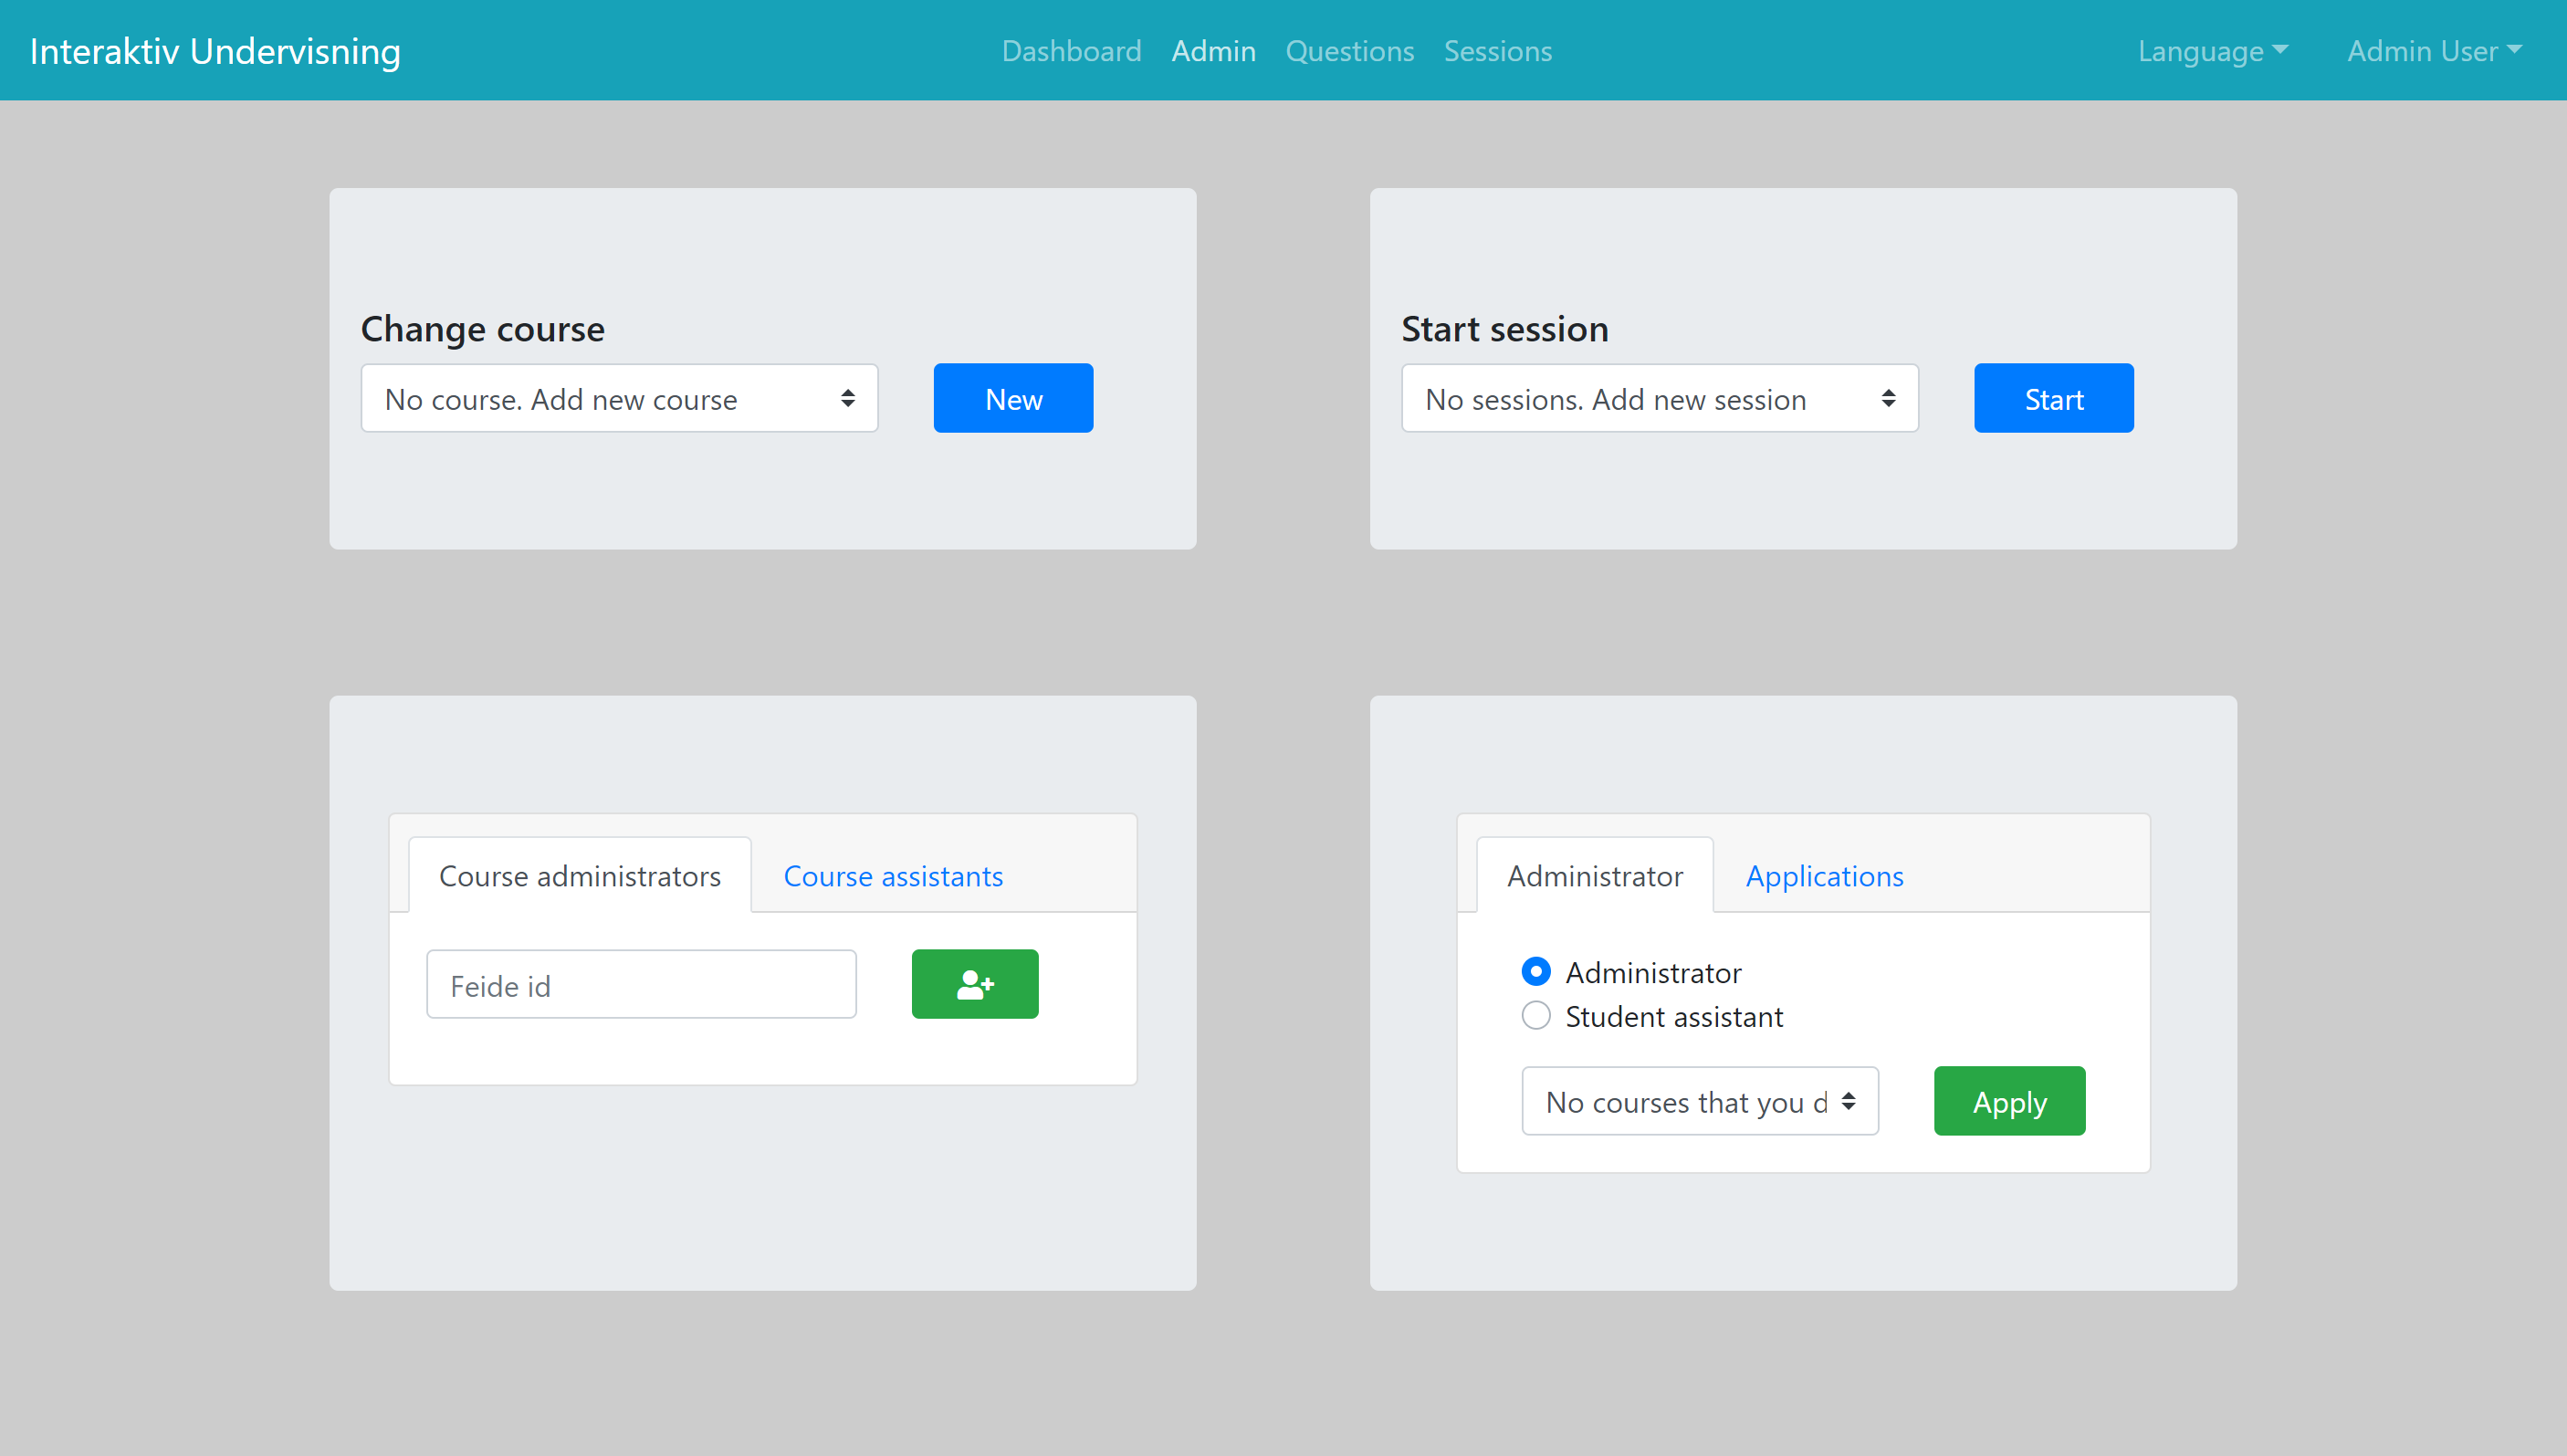
\includegraphics[width=0.80\linewidth]{/userManual/admin/Dashboard}
	\label{fig:adminDashboard}
	\caption{This figure displays the admin dashboard.}
\end{figure}